%% $Id: louveaux-epfl06.tex,v 1.5 2006/07/10 13:46:20 louveaux Exp $
%%\documentclass[9pt,trans]{beamer}
\documentclass[9pt,handout]{beamer}
\usepackage{beamerfoils}%% FoilTeX emulation
\usepackage{epsfig}
\usepackage{eurosym}
\mode<presentation>
{
  \usetheme{Boadilla}
  % oder ...

  \setbeamercovered{transparent}
  % oder auch nicht
}
\usepackage[french]{babel}
\usepackage[latin1]{inputenc}
%%\usepackage{times}
%%\usepackage[T1]{fontenc}
%\usepackage{booktabs}

%%\includeonlyframes{current}

\title{Discrete Optimization}

\author{Quentin
Louveaux}
\institute{ULg - Institut Montefiore}
\date{2016}

% Falls eine Logodatei namens "university-logo-filename.xxx" vorhanden
% ist, wobei xxx ein von latex bzw. pdflatex lesbares Graphikformat
% ist, so kann man wie folgt ein Logo einf|gen:

% \pgfdeclareimage[height=0.5cm]{university-logo}{university-logo-filename}
% \logo{\pgfuseimage{university-logo}}

% Folgendes sollte gelvscht werden, wenn man nicht am Anfang jedes
% Unterabschnitts die Gliederung nochmal sehen mvchte.
%% \AtBeginSection[]
%% {
%%   \begin{frame}<beamer>
%%     \frametitle{Gliederung}
%%     \tableofcontents[currentsection,currentsubsection]
%%   \end{frame}
%% }

% Falls Aufzdhlungen immer schrittweise gezeigt werden sollen, kann
% folgendes Kommando benutzt werden:

\beamerdefaultoverlayspecification{<+->}

%%%%%%
\definecolor{rot}{rgb}{1,0,0}
\definecolor{gruen}{rgb}{0,1,0}
\definecolor{blau}{rgb}{0,0,1}

%%% number sets
\newcommand{\Z}       {\mathbb{Z} }
\newcommand{\R}       {\mathbb{R} }
\newcommand{\Q}       {\mathbb{Q} }
\newcommand{\N}       {\mathbb{N} }
\newcommand{\spa}     {\text{span}}
\newcommand{\lin}     {\text{span}}
\newcommand{\inter}   {\text{int} }


%%% mathematical stuff
\newcommand{\sosR}    {\sum^2}
\newcommand*{\transpose}[1]  { {#1}^T }
\newcommand*{\rounddown}[1]  {\left\floor #1 \right\rfloor}
\newcommand*{\roundup}[1]    {\left\lceil  #1 \right\rceil}
\newcommand*{\ipart}[1]      {\rounddown{#1}}
\newcommand*{\fpart}[1]      {\mathfrak{f}\left(#1\right)}


\newcommand*{\iepoly}[2]  {z_{#1}\left(#2\right)}
\newcommand*{\redmon}[3]  {r_{#1}^{#2}\left( #3 \right)}
\newcommand*{\redset}[1]  {#1^{\emph{red}}}

\newcommand*{\Gpoly}[1] {P_{[#1]}}

\newcommand*{\nonc}[1]{\overline{#1}}
\newcommand*{\const}[1]{#1_0}

\newcommand{\define}{\stackrel{\rm def.}{\Leftrightarrow}}
\newcommand{\qform}[3]{\frac{1}{2} x^{\top}#1x + #2^{\top}x + #3}
\def\xzero{x^{0}}
\newcommand{\gxh}[2]{{g_{#1}(#2)}}

\def\pcone_k{{\mathcal C}_{k}(f)}
\def\orthant_j{{\mathcal O}_{j}}

\def\BDB{BDB^{\top}}
\def\LDL{LDL^{\top}}
\def\bA{A}
\def\bb{b}
\def\bc{c}
\def\bh{h}
\def\bp{p}
\def\bx{x}
\def\by{y}
\def\bu{u}
\def\bv{v}
\def\bd{d}
\def\T{^{T}}
\def\D{}
\def\mb{{\bf}}
\def\sep{}
\def\bo{0}
\def\bw{w}
\def\ba{a}
\def\bg{g}
\def\bH{H}
\def\be{e}

\let\ve=\relax
\newcommand\vealpha{{\alpha}}
\newcommand{\st}{\mathrm{s.t.}}
\DeclareMathOperator\conv{conv}
\DeclareMathOperator\cone{cone}
\newcommand{\B}{\{0,1\}}

\newcommand*{\person}[1] {\textsc{#1}}

\newtheorem{algorithm}{Algorithmus}

\makeatletter
\newenvironment{rmat}{\left(\null\,\vcenter\bgroup
  \Let@\restore@math@cr\default@tag
  \baselineskip6\ex@ \lineskip1.5\ex@ \lineskiplimit\lineskip
  \ialign\bgroup\hfil$\m@th\scriptstyle##$&&\thickspace
  \hfil$\m@th\scriptstyle##$\crcr
}{%
  \crcr\egroup\egroup\,\right)%
}
\makeatother

%%%%%%%%%%%%%%%%%%%%%%%%%%%%%%%%%%%%%%%%%%%%%%%%%%%%%%%%%%%%%%%%%%%%%%%%%%%%%%%%
%\begin{frame}
  %\titlepage
%\end{frame}

%% \begin{frame}
%%   \frametitle{Gliederung}
%%   \tableofcontents
%%   % Die Option [pausesections] kvnnte n|tzlich sein.
%% \end{frame}


%%%%%%%%%%%%%%%%%%%%%%%%%%%%%%%%%%%%%%%%%%%%%%%%%%%%%%%%%%%%%%%%%%

\definecolor{orange}{rgb}{0.8,0.3,0.0}
\definecolor{darkgreen}{rgb}{0.0,0.5,0.0}
\definecolor{gold}{rgb}{1.0,0.8,0.0}
\definecolor{brown}{rgb}{0.6,0.2,0.2}
\definecolor{blue4}{rgb}{0,0,144}
\definecolor{white}{rgb}{255,255,255}
\definecolor{blueexample}{rgb}{0.2,0.2,0.7}
\begin{document}
\begin{frame}
  \titlepage
\end{frame}
\begin{frame}
\frametitle{Modeling techniques}
We consider several concepts that can be well modeled
by \alert{integer programs}
\begin{block}{Binary choice}
A \alert{choice} between 2 alternatives is modeled through a 
$0,1$-variable.\\
\textcolor{blue}{Example}\\
The \alert{knapsack problem}
\begin{align*}
\text{maximize}\quad & \sum_{i=1}^n c_i x_i\\
\text{subject to}\quad& \sum_{i=1}^n a_i x_i \leq b\\
& x_i\in \{0,1\}\text{ for all }i=1,\ldots,n.
\end{align*}
\end{block}
\end{frame}
\begin{frame}
\frametitle{Modeling techniques}
\begin{block}{Forcing constraints}
\alert{If} decision $B$ is taken \alert{then} decision $A$ must be taken.
\begin{align*}
x=1\qquad & \text{if decision $A$ is taken}\\
x=0\qquad & \text{otherwise}\\
\\
y=1\qquad & \text{if decision $B$ is taken}\\
y=0\qquad & \text{otherwise}
\end{align*}
The constraint reads
\alert{$$y\leq x$$}
\textcolor{blue}{Example} Facility location problem
\end{block}
\end{frame}
\begin{frame}
\frametitle{Modeling techniques}
\begin{block}{Disjunctive constraints}
Consider $x\geq 0, a\geq 0, c\geq 0$.
We want to model an \alert{OR} constraint:
$$ a^T x \geq b \quad \text{or}\quad c^Tx \geq d $$
\uncover<2->{We introduce a variable $y\in \{0,1\}$
that represents whether \alert{constraint 1}
or \alert{constraint 2} is satisfied.\bigskip}
\uncover<3->{$$a^Tx\geq yb\quad \text{and}\quad c^Tx\geq (1-y)d.$$}
\end{block}
\end{frame}
\begin{frame}
\frametitle{Modeling techniques}
\begin{block}{Restricted range of values}
Suppose we want to formulate $x\in \{a_1,a_2,\ldots, a_m\}$.\bigskip

\uncover<2->{\noindent We introduce $m$ \alert{binary variables} $y_j$.\bigskip
$$x=\sum_{j=1}^m a_j y_j, \quad \sum_{j=1}^m y_j=1, \quad y_j\in\{0,1\}$$}
\end{block}
\end{frame}
\begin{frame}
\frametitle{Modeling techniques}
\begin{block}{Arbitrary piecewise linear cost functions}
\begin{center}
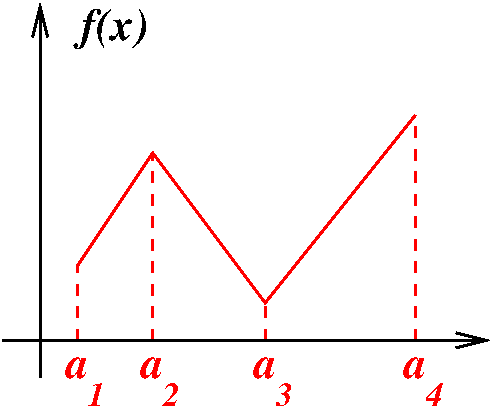
\includegraphics[width=.4\linewidth]{piecewise.pdf}
\end{center}
\uncover<2->{Introduce $y_i\in\{0,1\}$ such that
\begin{align*}
y_i=1\quad & \text{if } x\in[a_i,a_{i+1}]\\
y_i=0\quad & \text{if } x\not\in[a_i,a_{i+1}]
\end{align*}}
\end{block}
\end{frame}
\begin{frame}
\frametitle{Guidelines for strong formulation}
\begin{block}{The linear relaxation}
Given
\begin{align*}
\min\;& c^Tx+d^Ty\\
\text{s.t. }\;& Ax+By=b\\
&x,y\geq 0\\
&x\in\alert{\Z^n}.
\end{align*}
Its  \alert{linear relaxation} is defined as 
\begin{align*}
\min\;& c^Tx+d^Ty\\
\text{s.t. }\;& Ax+By=b\\
&x,y\geq 0\\
&x\in\alert{\R^n}.
\end{align*}
\end{block}
The linear relaxation gives important information about
the optimal value of an integer program.
\end{frame}
\begin{frame}
\frametitle{Reminder: linear programming}
If the objective is \alert{linear} and the constraints are \alert{linear},
we talk about \alert{linear programming} (LP) or \alert{linear optimization}.
\begin{block}{LP in standard form}
\begin{align*}
\min\; & c^T x\\
\st \;& Ax=b\\
& x\in \R^n_+
\end{align*}
\end{block}
\begin{block}{Definition}
A \alert{polyhedron} is a set $\{x\in \R^n|Ax\geq b\}$
\end{block}
A set of the      form  $Ax\leq b$ is also a polyhedron.\\
A set $\{x\in \R^n| Ax=b, x\geq 0\}$ is a polyhedron in \alert{standard form}.
\end{frame}
\begin{frame}
\frametitle{Graphic representation}
\only<1>{We can represent a problem in two dimensions graphically.\\
\textcolor{darkgreen}{Example:}}
\begin{alignat}{2}
\max \; x_1&+&2x_2 \label{objectif}\\
-x_1&+& 2x_2 & \leq 1  \label{contr2}\\
-x_1 &+& x_2  & \leq 0 \label{contr3}\\
4x_1 & +& 3x_2 &\leq 12 \label{contr4}\\
x_1&,&x_2&\geq 0 \label{nonneg}
\end{alignat}
\begin{overlayarea}{\linewidth}{5.5cm}
\begin{center}
\includegraphics<2>[width=5.2cm]{lp2d.pdf}
\includegraphics<3>[width=5.2cm]{feasibleregion.pdf}
\includegraphics<4>[width=5.2cm]{objectif1.pdf}
\includegraphics<5>[width=5.2cm]{objectif2.pdf}
\includegraphics<6>[width=5.2cm]{objectifoptimal.pdf}
\end{center}
\end{overlayarea}
\end{frame}
\begin{frame}
\frametitle{Extreme points and vertices}
\begin{block}{Definition}
Let $P$ be a polyhedron. A point $x\in P$ is an \alert{extreme point } of $P$ 
if there do not exist two   points $y,z\in P$ such that $x$ is a convex combination of
$y$ and $z$.
\end{block}
\vspace{2cm}
\begin{block}{Definition}
Let $P$ be a polyhedron. A point $x\in P$ is a \alert{vertex} of $P$ if
there exists  $c\in \R^n$ such that $c^Tx < c^T y$ for all $y\in P$ and  $y\neq x$.
\end{block}
\end{frame}
\begin{frame}
\frametitle{Degenerate cases}
In the example we had a \alert{unique solution} at a
\alert{vertex} of the \alert{polyhedron}.\\
Some degenerate cases can lead to different solutions.
%Dans l'exemple, on avait \alert{une solution unique} \`a un \alert{sommet} du \alert{poly\`edre}.\\
%Certains cas d\'eg\'en\'er\'es peuvent mener \`a diff\'erentes solutions.
\begin{overlayarea}{\linewidth}{2cm}
\only<2>{
\begin{align*}
\min\; & x_1 + x_2\\
\text{s.t. } & -x_1+x_2 \leq 1\\
& x_1,x_2\geq 0
\end{align*}}
\only<3>{
\begin{align*}
\min\; & x_1 \\
\text{s.t. } & -x_1+x_2 \leq 1\\
& x_1,x_2\geq 0
\end{align*}}
\only<4>{
\begin{align*}
\max\; & -x_1+x_2 \\
\text{s.t. } & -x_1+x_2 \leq 1\\
& x_1,x_2\geq 0
\end{align*}}
\only<5>{
\begin{align*}
\max\; & x_1+x_2 \\
\text{s.t. } & -x_1+x_2 \leq 1\\
& x_1,x_2\geq 0
\end{align*}}
\only<6>{
\begin{align*}
\max\; & x_1+2x_2 \\
\text{s.t. } & -x_1+x_2 \leq 1\\
&-x_1+x_2 \geq 2\\
& x_1,x_2\geq 0
\end{align*}}
\end{overlayarea}
\begin{overlayarea}{\linewidth}{5cm}
\begin{center}
\includegraphics<2>[width=5cm]{uniqueoptimal.pdf}
\includegraphics<3>[width=5cm]{boundedoptimal.pdf}
\includegraphics<4>[width=5cm]{unboundedoptimal.pdf}
\includegraphics<5>[width=5cm]{nooptimal.pdf}
\includegraphics<6>[width=5cm]{infeasible.pdf}
\end{center}
\end{overlayarea}
\end{frame}
\begin{frame}
\frametitle{Bases of a polyhedron}
%On consid\`ere les diff\'erentes \'egalit\'es et in\'egalit\'es 
%en trois cat\'egories:
We subdivide the equalities and inequalities into three categories:
\begin{align*}
a_i^T x \geq b_i \qquad & i\in M_{\geq}\\
a_i^T x \leq b_i \qquad& i \in M_{\leq}\\
a_i^T x = b_i \qquad& i \in M_{=}
\end{align*}
\begin{block}{Definition}
Let  $\bar x$ be a point satisfying  $a_i^T \bar x = b_i$ for some  $i\in M_{\geq}, M_{\leq}$ or
$M_=$. The constraint $i$ is said to be \alert{active} or \alert{tight}.
\end{block}
\end{frame}
\begin{frame}
\frametitle{Bases of a polyhedron}
\begin{block}{Definition}
Let  $P$ be a polyhedron and let $\bar x \in \R^n.$
\begin{enumerate}[(a)]
\item<1-> $\bar x$ is a \alert{basic solution} if 
\begin{itemize}
\item<1-> all equalities ($i\in M_=$) are \alert{active}
\item<1-> among the active constraints, there are \alert{$n$ linearly 
independent} 
\end{itemize}
\item<1-> if $\bar x$ is a basic solution  \alert{that satisfies all constraints}, then
$\bar x$ is a \alert{feasible basic solution}.
\end{enumerate}
\end{block}
\begin{block}{Theorem}
Let  $P$ be a polyhedron and let  $\bar x \in P$. The three following statements are
equivalent.
\begin{enumerate}[(i)]
\item<2-> $\bar x$ is a \alert{vertex}
\item<2-> $\bar x$ is an \alert{extreme point}
\item<2-> $\bar x$ is a \alert{basic feasible solution}
\end{enumerate}
\end{block}
\end{frame}
\begin{frame}
\frametitle{Main messages}
\begin{itemize}
\item The problem
\begin{align*}
\min\; & c^T x\\
\text{subject to } & a_{(i)}^T x \leq b_{(i)}\qquad i=1,\ldots, m\\
& x\in \alert{\mathbb{R^n_+}}
\end{align*}
can be solved efficiently both \alert{in theory} and in \alert{practice}.\\
Problems with \alert{thousands} of variables and constraints can be solved in \alert{seconds}.\medskip
\item \alert{An} optimal solution can always be found among \alert{vertices}\medskip
\item The \alert{simplex algorithm} always outputs a \alert{vertex} as an optimal solution.\medskip
\item If you \alert{add a new constraint to the problem}, you can \alert{reoptimize} very quickly using the simplex algorithm.
\end{itemize}
\end{frame}

\end{document}
\begin{frame}
\frametitle{Comparing two formulations}
To compare \alert{two formulations} $P^1$ and $P^2$ with
the same \alert{integer feasible points}, we consider
their respective \alert{linear relaxations} $P^1_{LP},P^2_{LP}$.
\bigskip

\uncover<2->{\begin{block}{Comparing two formulations}\noindent $P^1$ is \alert{better} than $P^2$ 
if $$P^1_{LP} \subset P^2_{LP}$$\end{block}}

\uncover<3->{\begin{block}{Ideal formulation}
If $\mathcal F=\{x_1,\ldots,x_k\}$ is the set of
\alert{feasible solutions}, an \alert{ideal formulation} is
$$\conv(\mathcal F)$$\end{block}\bigskip

\noindent
\textcolor{blue}{Example}: The facility location problem}\bigskip

\noindent
\textcolor{blue}{Example:} The pigeonhole principle

\end{frame}
\begin{frame}
\frametitle{Comparing two formulations for graph problems}
\begin{block}{The minimum spanning tree}
Let $G=(V,E)$ be an undirected graph. Every edge has a \alert{cost $c_e$}.
We look for the tree with the \alert{minimum total cost}.
\begin{overlayarea}{\linewidth}{4cm}
\begin{center}
\includegraphics<1>[width=.3\linewidth]{mst1.pdf}
\includegraphics<2->[width=.3\linewidth]{mst2.pdf}
\end{center}
\end{overlayarea}
\end{block}
\uncover<3->{Constraints to encode:}
\begin{itemize}
\item<4-> A tree should have \alert{$n-1$ edges} where $n$ is the number of nodes
\item<5-> A tree \alert{cannot have a cycle} or equivalently\\
A tree must be \alert{connected}
\end{itemize}
\end{frame}
\begin{frame}
\frametitle{Subtour elimination formulation}
\begin{block}{Integer formulation}
\begin{align*}
P^I_{sub} = \{ x_e \in \{0,1\} \mid & \sum_{e\in E} x_e=n-1\\
& \sum_{e\in E(S)} x_e \leq |S|-1, \quad S\subset V, S\neq \emptyset, V\;\}
\end{align*}
\end{block}
\begin{block}{Linear programming relaxation}
\begin{align*}
P_{sub} = \{ x_e \in \alert{[}0,1\alert{]} \mid & \sum_{e\in E} x_e=n-1\\
& \sum_{e\in E(S)} x_e \leq |S|-1, \quad S\subset V, S\neq \emptyset, V\;\}
\end{align*}
\end{block}
\end{frame}
\begin{frame}
\frametitle{Cutset  formulation}
\begin{block}{Integer formulation}
\begin{align*}
P^I_{cut} = \{ x_e \in \{0,1\} \mid & \sum_{e\in E} x_e=n-1\\
& \sum_{e\in \delta(S)} x_e \geq 1, \quad S\subset V, S\neq \emptyset, V\;\}
\end{align*}
\end{block}
\begin{block}{Linear programming relaxation}
\begin{align*}
P_{cut} = \{ x_e \in \alert{[}0,1\alert{]} \mid & \sum_{e\in E} x_e=n-1\\
& \sum_{e\in \delta(S)} x_e \geq 1, \quad S\subset V, S\neq \emptyset, V\;\}
\end{align*}
\end{block}
\end{frame}
\begin{frame}
\frametitle{Comparing the two formulations}
\begin{block}{Theorem}
\begin{itemize}
\item $P_{sub}\subset P_{cut}$ and the inclusion is sometimes strict
\item $P_{cut} $ can have fractional extreme points
\end{itemize}
\end{block}
\end{frame}
\begin{frame}
\frametitle{The traveling salesman problem}
\begin{block}{Subtour elimination formulation}
\begin{align*}
P^I_{tspsub} = \{ x_e \in \{0,1\} \mid & \sum_{e\in \delta(\{i\})} x_e=2\quad \text{for all }i\in V\\
& \sum_{e\in E(S)} x_e \leq |S|-1, \quad S\subset V, S\neq \emptyset, V\;\}
\end{align*}
\end{block}
\begin{block}{Cutset formulation}
\begin{align*}
P^I_{tspcut} = \{ x_e \in \{0,1\} \mid & \sum_{e\in \delta(\{i\})} x_e=2 \quad \text{for all } i\in V\\
& \sum_{e\in \delta(S)} x_e \geq 2, \quad S\subset V, S\neq \emptyset, V\;\}
\end{align*}
\end{block}
\begin{block}{Theorem}
If $P_{tspsub} $ and $P_{tspcut}$ are the respective linear relaxations,
$$P_{tspsub}=P_{tspcut}$$
\end{block}
\end{frame}
\end{document}
